\section{Future Work}
\label{sec:future_work}

% needs updating since we include subject 2

Our future work will extend our experiments from solely NSD subject 1 to the full four-subject setting which other papers use. This would evaluate whether the observed performance of our pipeline holds up across all subjects with differing brain anatomies.

We would likely implement this by introducing a shared functional clustering space across subjects. Specifically, we would summarize each flatmap patch across trials into a single description vector, then fit a Gaussian Mixture Model \cite{dempster1977maximum} to map brain patches from all subjects into a common cluster space. A cross-attention layer could then compress the patches assigned to each cluster into a fixed set of cluster tokens. Similar strategies have proven effective in prior work for training a single transferable model across many subjects.

Together, these extensions would enable a more direct comparison against prior multi-subject methods and test whether our approach remains competitive at scale.

Another direction is to replace CLIP as the target semantic representation, with an embedding space from more recent model such as SigLIP2 \cite{tschannen2025siglip2multilingualvisionlanguage}. One limitation is that semantic conditioning with the CLIP embeddings comes at the expense of our low-level performance. Replacing CLIP with a stronger semantic embedding model such as SigLIP2 could improve our visual-semantic alignment, and subsequent performance on both low-level and high-level evaluations. This may require training an SDXL decoder that accepts SigLIP2 embeddings as conditioning inputs.

\begin{figure}[!t]
\centering
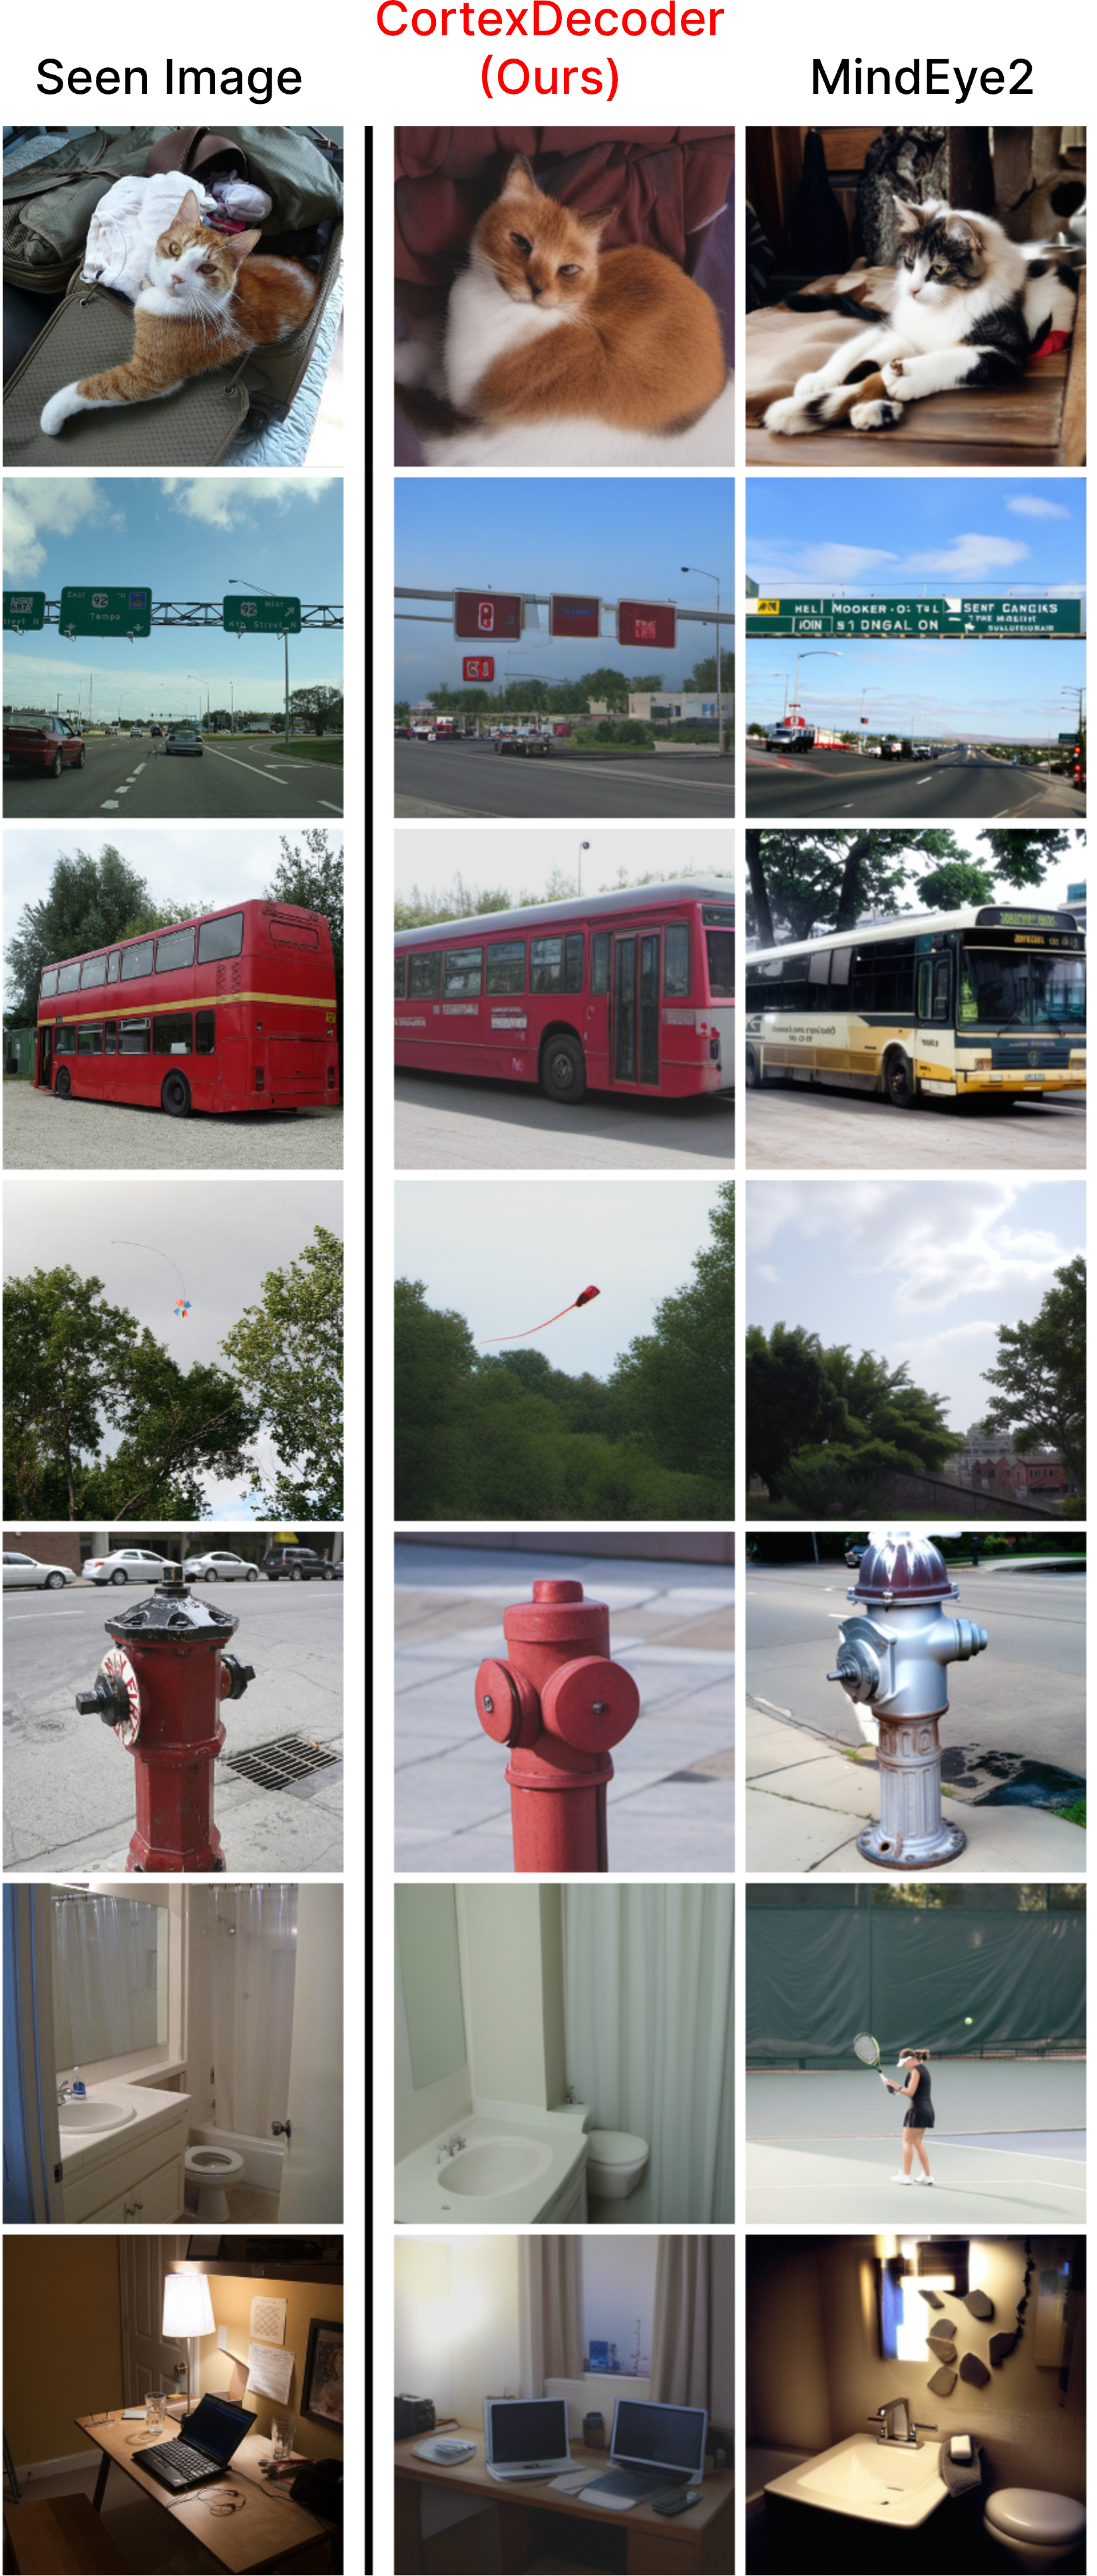
\includegraphics[width=0.8\columnwidth]{images/comparison4.png}
\caption{Image reconstructions comparing models. The left column shows the original image stimuli, middle column is our model, and rightmost column is MindEye2 generations. Each row corresponds to a reconstruction of the same image stimulus. Images including those depicting faces are derived from the Microsoft COCO dataset, used under CC-BY 4.0. \cite{lin2015microsoftcococommonobjects}}
\label{fig:comparison}
\end{figure}
